\documentclass[conference]{IEEEtran}
\usepackage{xcolor}
\usepackage{cite}
\usepackage{url}
\usepackage{graphicx}
\usepackage{enumitem}
\usepackage{parskip}

\begin{document}
\newcommand{\derek}[1] {\textcolor{blue}{\textbf{[Derek: #1]}}}
\newcommand{\mina}[1] {\textcolor{green}{\textbf{[Mina: #1]}}}
\newcommand{\mazyar}[1] {\textcolor{orange}{\textbf{[Mazyar: #1]}}}
\newlist{questions}{enumerate}{2}
\setlist[questions,1]{label=RQ\arabic*.,ref=RQ\arabic*}
\setlist[questions,2]{label=(\alph*),ref=\thequestionsi(\alph*)}

\title{Phylogenetic and Structural Analysis of BC200 and Hominoidea Homologs}

\author{Derek Robinson, Mina Emadi, Mazyar Ghezelji\\
University of Victoria\\
Victoria, Canada \\
\{drobinson, minaemadi, mazyarghezelji\}@uvic.ca}

\maketitle

\section{Introduction}\label{sec:intro}

Alzheimer's disease (AD) is a neurodegenerative disease which greatly affects the lives of those who are diagnosed and those who care for the diagnosed. 
In the United States, 6.2 million patients are estimated to be living with AD and it is the sixth leading cause of death for American adults \cite{AlzheimersDisease}. 
In Canada, over 747,000 patients are living with AD, or another form of dementia \cite{ADcanada}. 
Symptoms of AD range from memory loss and poor judgement in mild cases to the inability to communicate and seizures in severe cases \cite{alzheimersSigns}.

AD involves multiple cell types and signaling pathways \cite{zhang2021role}, as such, the collective knowledge of AD is spread across many different domains. 
This spread of knowledge means that fully understanding AD in humans is difficult, let alone understanding the disease in other species of the hominoidea superfamily.
Finch and Austad argue that with our current understanding of AD, it is not possible to determine if AD is uniquely human \cite{finch2015commentary}. 
As such, this paper explores one facet of AD pathogenesis, the long non-coding RNA (lncRNA) BC200. 
BC200 has been implicated in AD as it upregulates the expression of b-site APP-cleaving enzyme1 (BACE1) \cite{li2018identification,zhang2021role}. 
The upregulation of BACE1 in turn leads to higher levels of beta-amyloid (A$\beta$) in the brain, thus, disrupting cell function \cite{li2018identification,zhang2021role}. 

In hopes of better understanding how AD may affect other species in the hominoidea superfamily, specifically, the role that hominoidea homologs of BC200 play in AD, we answer the following research questions:

\begin{questions}
  \item What does the phylogenetic tree of BC200 look like?
  \item What structural differences exist between BC200 and its four most closely related hominoidea homologs?
\end{questions}

The following paper is structured as follows: section \ref{sec:background} gives background into BC200 and the role it plays in AD, section \ref{sec:methods} lays out the methods used for selecting BC200 homologs and performing both the phylogenetic structural analysis, section \ref{sec:results} presents the results of our analysis, section \ref{sec:discussion} discusses the relevancy of the results, and section \ref{sec:conclusion} concludes the paper.

\section{Background}\label{sec:background}

\subsection{What is BC200?}

Brain Cytoplasmic 200 lncRNA RNA (BC200) is a 200 nucleotide long RNA transcript which is found mostly in the brain \cite{tiedge1993primary}. 
As a non-coding RNA, BC200 is not translated into protein but can be used as a potential therapeutic target and biomarker due to its regulatory role in biological processes involved in disease development \cite{zhang2021role,mus2007dendritic}. 
This lncRNA has recently been studied extensively because of its role in regulating translation and inhibiting its initiation, as well as its impacts in the pathogenesis of Alzheimer's disease and cancer \cite{zhang2021role,tiedge1993primary}. 
These \derek{these being BC200?} non-coding RNAs are involved in translation control, thus, they impact the synthesis of dendritic proteins which facilitates long-term plastic changes at the synapse \cite{mus2007dendritic}.

\subsection{The Relation Between AD and BC200}

Alzheimer's disease (AD) is a neurodegenerative disease resulting from synaptic plasticity failure in neurons \cite{mus2007dendritic}. 
It is a complex disease, meaning that it involves multiple cell types and signaling pathways \cite{zhang2021role}.

AD is thought to occur due to the accumulation of two proteins in the brain. 
One of them is beta-amyloid (A$\beta$) which accumulates in neurons, forms plaques, and disrupts cell functions. 
The other one is hyper-phosphorylated tau protein which in abnormal levels can form neurofibrillary tangles in neurons and block synaptic transmissions \cite{zhang2021role}.

A$\beta$, a cleavage product of the amyloid precursor protein (APP), is generated by b-site APP-cleaving enzyme1 (BACE1) and $\gamma$-secretase complex, and it strongly influences the pathogenesis of AD. 
Inhibition of BACE1 activity and the subsequent reduction in A$\beta$ levels may cure or prevent AD\cite{li2018identification,zhang2021role}.

BC200 facilitates AD pathogenesis by up-regulating A$\beta$ production through the modulation of BACE1 expression. 
The inhibition of BC200 significantly suppresses BACE1 expression, increases cell viability and reduces cell apoptosis in an AD model, and these effects are reversed by BC200 over-expression \cite{li2018identification,zhang2021role}.

Many researches have demonstrated the important role of BC200 in AD. 
El Mus \emph{et al.} \cite{mus2007dendritic} show that there are steady decline in BC200 level from age 49 to 86, but, in AD brain its level was substantially higher. 
They also observe that BC200 expression is increased in brain areas that are involved in AD and it is parallel with severity of disease. 
Huanyen Li \emph{et al.} \cite{li2018identification} establish an AD cell model overexpressing A$\beta$1-42 to observe the effects of BC200 on the cell viability and apoptosis and to investigate the associated underlying mechanisms. 
They observe that BC200 and BACE1 were increased upon treatment with A$\beta$1-42, and inhibition of BC200 rescued this A$\beta$1-42-mediated dysfunction, as indicated by the interaction of BC200 directly targeting BACE1. 
Moreover, inhibition of BC200 increased AD cell growth and reduced cells apoptosis. 
They demonstrate that BC200 is a potent positive regulator of BACE1 in AD cells and in conclusion, lncRNA BC200 facilitates AD pathogenesis by up-regulating A$\beta$ through BACE1.  					 			 		 	 

\section{Materials and Methods}\label{sec:methods}

\subsection{Selection of lncRNAs}
The lncRNA BC200 was selected for phylogenetic analysis due to the role it plays in AD as discussed in section \ref{sec:background}. 
The homologs of BC200 were selected as a result of an NCBI Blast \cite{blastTool}. Specifically, Megablast \cite{morgulis2008database} with default parameters was used as it is able to compare closely related sequences \cite{amirmahani2018phylogenetic}. 
From the Blast results, sequences which are known BC200 homologs as indicated by the inclusion of BC200 in their name were chosen. 
Table \ref{tbl:accession} outlines the organism, sequence name, and accession number of each of the chosen sequences. 



\section{Results}\label{sec:results}

\subsection{Phylogenetic Tree of BC200}
TODO

\subsection{Structural difference between BC200 and its homologs}

Brain cytoplasmic 200 long non-coding RNA (or BC200 lncRNA) is a 200 nucleotide RNA transcript that is found predominantly in the brain. It's primary function is regulating translation by inhibiting its initiation.
It's role in AD is not fully understood, but research shows that Long noncoding RNA BC200 facilitates AD pathogenesis by upregulating AB through BACE1.Pathologically, AD is characterized by an imbalance in the production and clearance of amyloid-beta in the brain leading to plaque formation.\cite{li2018identification}
The BC200 structure consist of three main parts: A-rich domain, Alu domain and unique domain \cite{jung2014rna}.
\begin{figure}
  \centering
  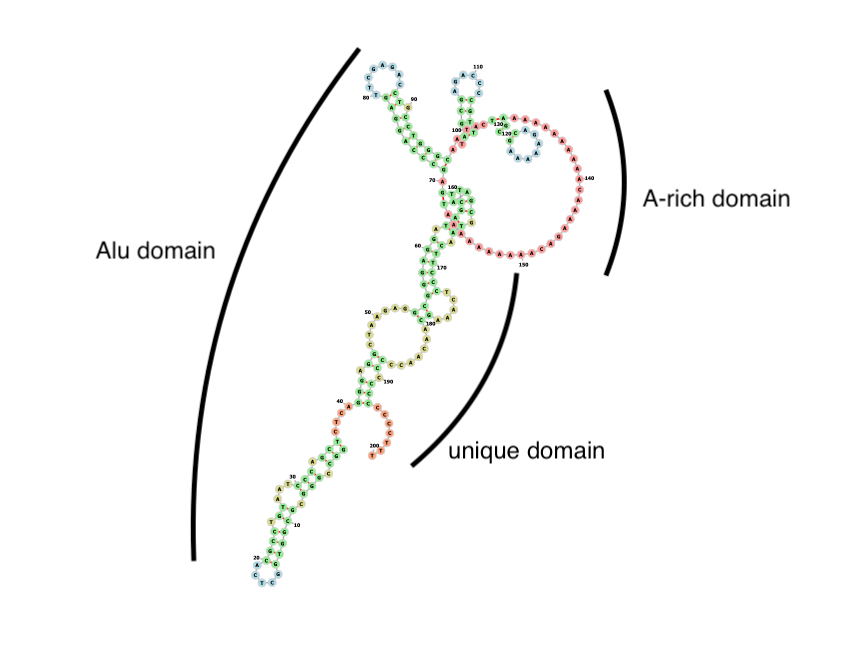
\includegraphics[width=0.4\textwidth]{figs/rna-6.png}
  \caption{BC200 RNA Secondary Structure}
\end{figure}
As we can see from the RNA secondary structures, all of the homologs have a nearly simialr A-rich domain, but on the other hand the the Alu domain is different between the homologs and BC200. The Alu domain of the mammalian signal recognition particle (SRP) comprises the heterodimer of proteins SRP9 and SRP14 bound to the 5′ and 3′ terminal sequences of SRP RNA\cite{weichenrieder2000structure}. So, their function in brain should be very different with eachother, eventhough there may be high similarity between their sequences. Here we have the three most related homologs that are great apes and one homolog which is not a great ape, but since it was in the three most related homologs to BC200 based on phylogenetic tree, we investigate its structure as well.

\begin{figure}
  \centering
  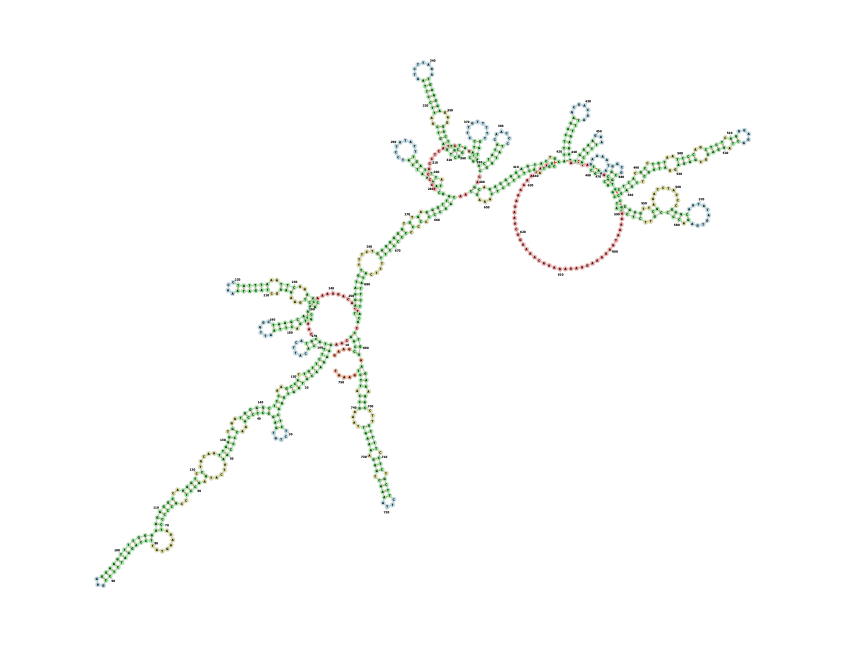
\includegraphics[width=0.4\textwidth]{figs/rnagorilla.png}
  \caption{BC200 RNA Secondary Structure in Gorilla}
\end{figure}
\begin{figure}
  \centering
  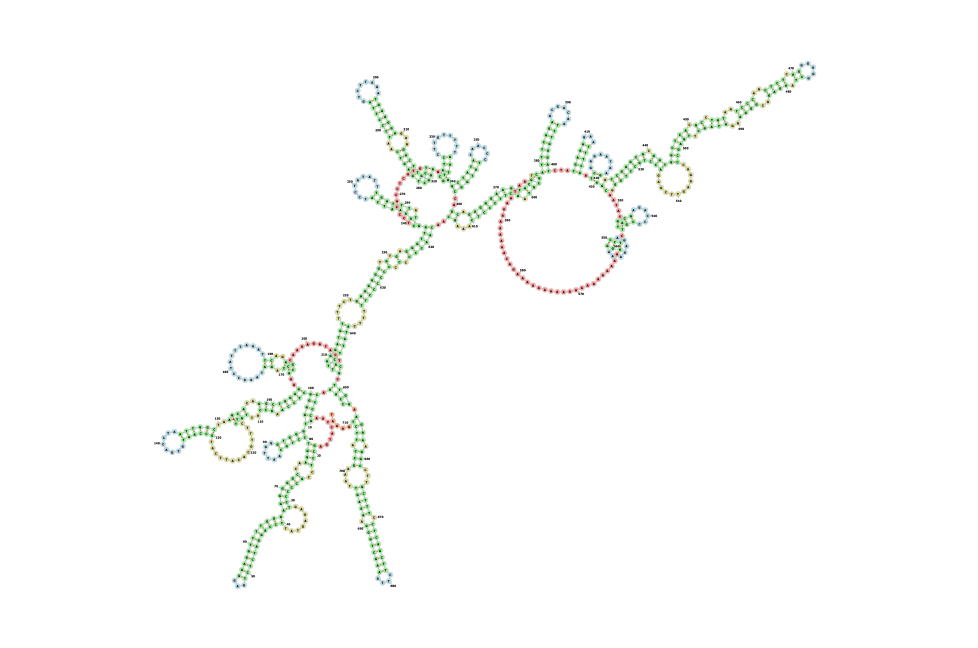
\includegraphics[width=0.4\textwidth]{figs/rnapan.png}
  \caption{BC200 RNA Secondary Structure in Pan}
\end{figure}
\begin{figure}
  \centering
  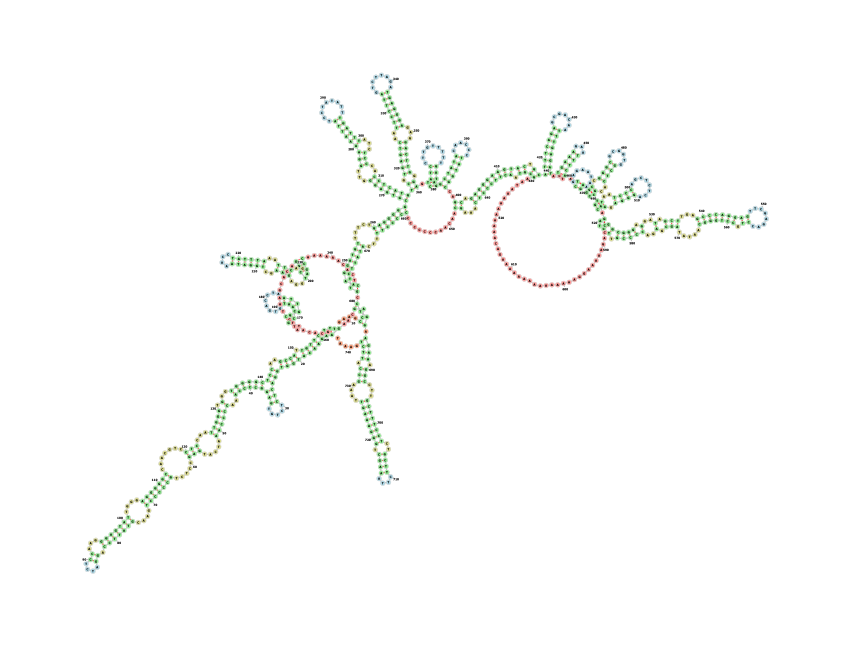
\includegraphics[width=0.4\textwidth]{figs/rnapango.png}
  \caption{BC200 RNA Secondary Structure in Pango}
\end{figure}

\begin{figure}
  \centering
  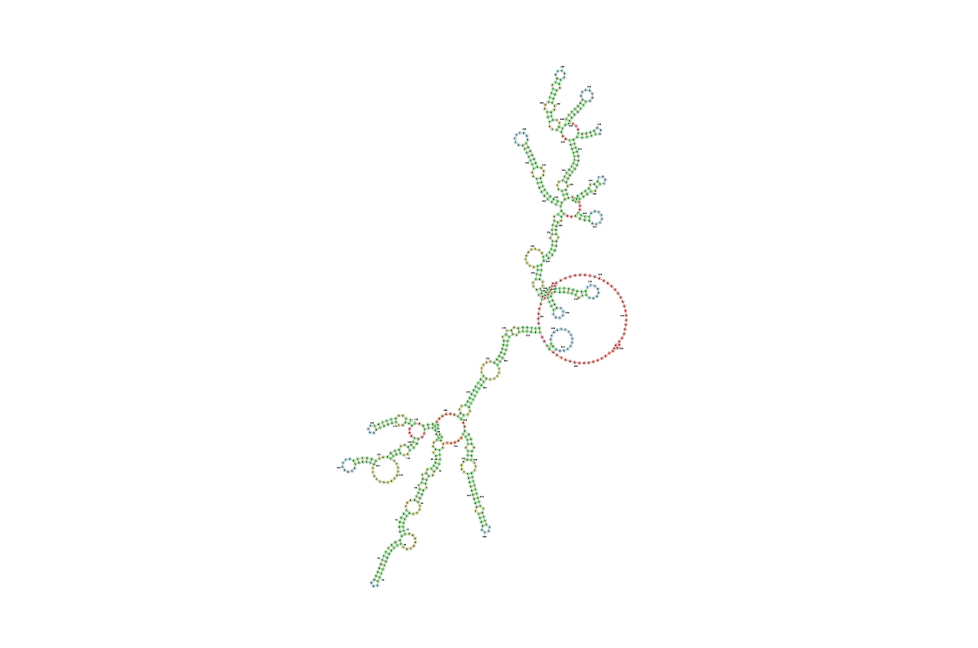
\includegraphics[width=0.4\textwidth]{rna.png}
  \caption{BC200 RNA Secondary Structure in Hylobates lar}
\end{figure}
\subsection{Comparing BC200 sequence with its homologs}


\subsection{Comparing BC200 sequence with its homologs}

One of the best ways for finding the conserved portions of a gene during evolution, is sequence alignment. Here, we aligned BC200 and the three most related homologs with each other to find the conserved parts of the sequence.

Here are the alignment results:
\begin{figure}
  \centering
  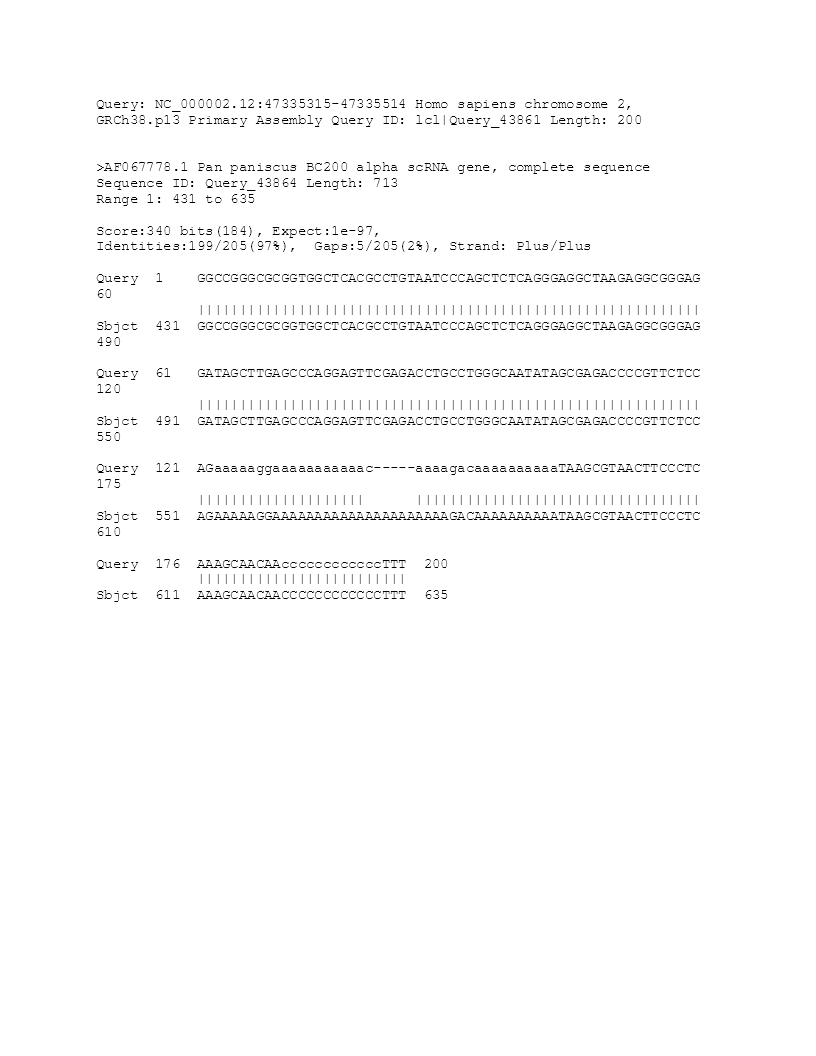
\includegraphics[width=0.4\textwidth]{figs/TK1PBYHT114-Alignment-2-page-1.png}
  \caption{BC200 Sequence Alignment with BC200 in pan}
\end{figure}
\begin{figure}
  \centering
  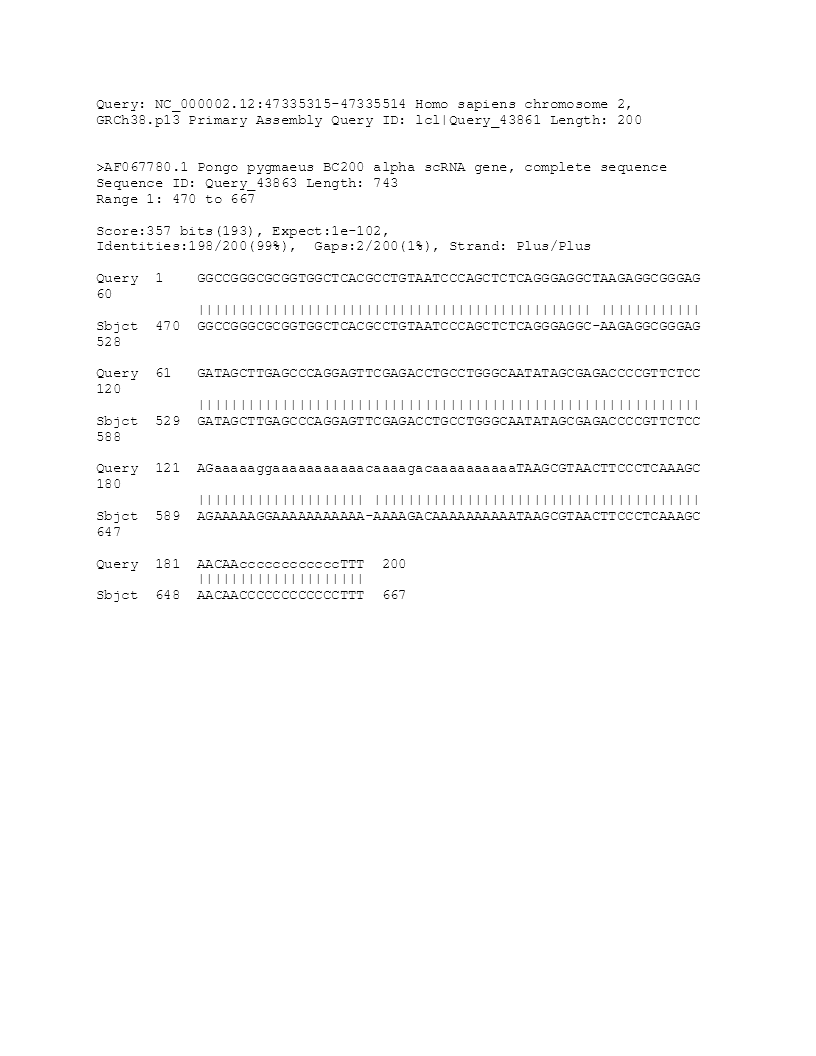
\includegraphics[width=0.4\textwidth]{figs/TK1PBYHT114-Alignment-3-page-1.png}
  \caption{BC200 Sequence Alignment with BC200 in Pango}
\end{figure}
\begin{figure}
  \centering
  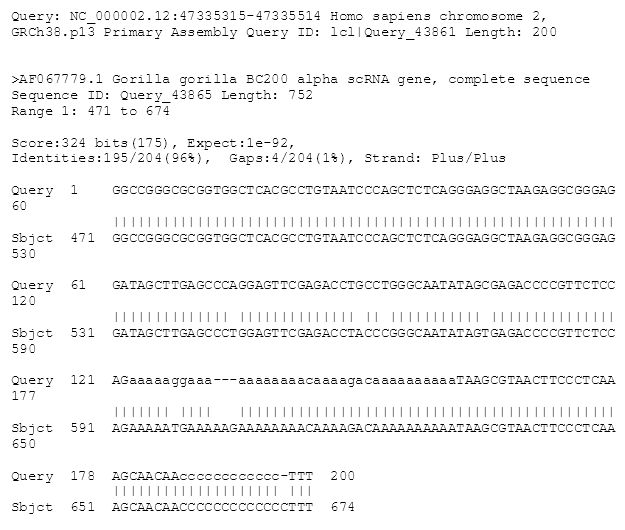
\includegraphics[width=0.4\textwidth]{figs/TK1PBYHT114-Alignment-page-1.png}
  \caption{BC200 Sequence Alignment with BC200 in Gorilla}
\end{figure}

As it is obvious from the results, most parts of the sequence are conserved. Which shows that there should be a high similarity between BC200 RNA in human body and in other species. So, the following result does not support our hypothesis, and they suggest that Alzheimer’s can be shared between human and great apes.

\section{Discussion}\label{sec:discussion}
TODO

\section{Conclusion}\label{sec:conclusion}
TODO

\bibliographystyle{IEEEtran}
\bibliography{refs.bib}
\end{document}
